\documentclass[sigconf,nonacm]{acmart}
\bibliographystyle{ACM-Reference-Format}

\AtBeginDocument{%
  \providecommand\BibTeX{{%
    \normalfont B\kern-0.5em{\scshape i\kern-0.25em b}\kern-0.8em\TeX}}}

%% Rights management information.
\setcopyright{acmcopyright}
\copyrightyear{2020}
\acmYear{2020}
%% \acmDOI{}
\acmConference[FWPM:Angewandtes maschinelles Lernen]{Angewandtes maschinelles Lernen}{Sommersemester, 2020}{Hof}
\acmBooktitle{FWPM:Angewandtes maschinelles Lernen, Sommersemester, 2020, Hof}
\acmPrice{}
\acmISBN{}

%% Additional Packages
\usepackage[ngerman]{babel}
\usepackage{graphicx}

%% Additional Modifications
\settopmatter{printacmref=false}
\graphicspath{ {./images/} }

\usepackage{listings}
\lstset{
  breaklines=true,
  literate=%
  {Ö}{{\"O}}1
  {Ä}{{\"A}}1
  {Ü}{{\"U}}1
  {ß}{{\ss}}1
  {ü}{{\"u}}1
  {ä}{{\"a}}1
  {ö}{{\"o}}1
}

\begin{abstract}
In dieser Studienarbeit wird die Performance unterschiedlicher strukturierter Reinforcement-Learning (kurz: RL) Modelle innerhalb einer \textit{Super Mario Bros.} (1985) \cite{wiki:smb} (kurz: SMB) Umgebung hinsichtlich ihrer Lernperformance und -stabilität auf Basis eines Experiments untersucht.

Konkret werden unterschiedliche RNN-Architekturen mit unterschiedlichen \textit{CNN}-Architekturen hinsichtlich ihres Performance bei limitierter Hardware verglichen. Dazu musste sich zunächst auf einen RL-Algorithmen geeinigt werden und anschließend das Neuronale Netzwerk und dessen Hyperparameter optimiert werden.

Abschließend wird das Ergebnisse des Projekts diskutiert.

Der Quellcode für das Projekt und sowie dessen Ergebnisse stehen öffentlich als Repository zur Verfügung \cite{selfgit}.
\end{abstract}

%% end of the preamble
\begin{document}

%% title
\title{Deep-Q-Learning mit 'Super Mario Bros' und A3C.}

%% author
\author{Jan Bernd Gaida}
\email{jan.gaida@hof-university.de}
\affiliation{
    \institution{Hochschule für Angewandte Wissenschaften Hof}
    \streetaddress{Alfons-Goppel-Platz 1}
    \city{Hof an der Saale}
    \state{Bavaria}
    \country{Germany}
    \postcode{95028}
}

\maketitle

\section{Einführung}
Maschinelles Lernen ist die Wissenschaft Computer indirekt zu programmieren. In der vergangen Dekade ist der Einsatz solcher Programme so allgegenwärtig geworden, das Vielen ihre eigentliche Verwendung nicht bewusst ist obwohl Sie mehrmals täglich verwendet wird. \cite{andrewWhatIs}

Reinforcement-Learning ist ein junger Teilbereich des Maschinelle Lernens, bei dem das Programm eine Umgebung eigenständig erkundet und in Abhängigkeit des Problems eine konkrete Lösung definiert. Dieses Verständnis erlangt das Programm mittels '\textit{Reinforcement}' (deutsch: bekräftigende, bestätigende) Mechanismen.

Medienwirksame Aufmerksamkeit erlangt dieser Teilbereich durch beeindruckende Rekorde oder Siege in sehr komplexen Spielen wie beispielsweise '\textit{AlphaGo}', das erste Computerprogramm das einen menschlichen Spieler im dadurch berühmten Brettspiel \textbf{Go} besiegte \cite{alphago}. Oder beispielsweise die künstliche Intelligenz '\textit{OpenAI Five}' die das Multiplayerspiel \textit{Dota 2} auf Experten Niveau spielt \cite{openaifive}.

Auch wenn dieser Bereich scheinbar keine konkreten Verbesserungen für das alltägliche Leben birgt, bietet das experimentieren mit solchen komplexen künstlich geschaffenen Umgebungen ein großer Forschungspotential. Dies wird langfristig dazu führen, dass vor allem Roboter in weniger komplizierten Anwendungsbereichen, wie beispielsweise dem korrekten Sortieren von Objekten von Laufbändern, großer Fortschritt machen wird \cite{awbrl}.

Das Potential von Reinforcement-Learning ist also groß und wird uns sicherlich auch weiterhin dazu Anregen, dieses weiter zu entwickeln und im Alltag nutzbar zu machen.

\section{Hardware}
\label{hardware}
Das Training des Modells fand auf einem \textit{Consumer-Pc} statt. Konkret standen hierfür 6 GB VRAM (\textit{GeForce GTX 1060}) erreichbar mittels \textit{CUDA}-Treiber, sowie 16 GB RAM (DDR3 im Dual-Channel Modus bei ca. 800 MHz Frequenz) unterstützt durch eine 4 Kern CPU getaktet auf ca. 3.8 GHz (\textit{Intel Core i5 4690K}). Genannte Hardware wurde zum Trainigs- und Testzeitpunkt moderat übertaktet.

\section{Lern- und Testumgebung}
Als Laufzeit- und Entwicklungsumgebung wurde Python 3.8 (offizielle Releaseversion) gewählt. Nachfolgend werden die wesentlichen benutzten Frameworks kurz aufgeführt, welche allesamt mittels Pip-Paketmanager installierbar sind.

\subsection{OpenAI Gym und SMB-Gym}
\label{smbgym}
\textit{OpenAI Gym} \cite{Brockman2016OpenAIG} ist ein bekanntest Framework zum trainieren und testen unterschiedlicher RL-Algorithmen. Ziel der Entwickler ist es hierbei für diesen Algorithmentypus eine standardisierte Umgebung, meist als Enviorment bezeichnet, zur bessere Vergleichbarkeit mit ähnlichem anzubieten. Dadurch eignet sich dieses Framework bestens für sog. Benchmarktests mit weiteren RL-Algorithmen, mit denen Vor- und Nachteile dieser Algorithmen analysiert und interpretiert werden können.

Durch die Machine-Learning-Community gibt es eine große Anzahl an verfügbaren '\textit{Gyms}', wie das in diesem Projekt genutzte: '\textit{Super Mario Bros for OpenAI Gym}' \cite{gym-smb}. Dieses ist ein von Christian Kauten zur Verfügung gestelltes SMB-Enviroment, welches die letzte Version von \textit{OpenAI Gym} (Stand: 2020) unterstützt und weitere Features beinhaltet. So werden in diesem \textit{Gym} unterschiedliche Render-Versionen und vordefinierte Eingabekombination (sog. ActionSpace) angeboten (vgl. \ref{smbconfig}).

Zur Verfügung steht dieses Enviorment aus urheberrechtlichen Gründen nur für Bildungszwecke, vgl. \textit{Digital Millennium Copyright Act} (kurz: \textit{DMCA}) \cite{dmca}.

\subsection{PyTorch}
Als Machine-Learning-Framework wurde \textit{PyTorch} \cite{pytorch}, ein bekanntes und speichereffizientes open source Framework, verwendet. Dieses wurde ursprünglich von einem \textit{Facebook}-Forschungsteam für künstliche Intelligenz entwickelt und basiert auf der in \textit{Lua} geschriebenen Bibliothek \textit{Torch} \cite{torch}. \cite{pytorchtext}

\subsection{Tensorboard und Ähnliche Bibliotheken}
Zur Visualisierung der Lernergebnisse wurde \textit{Tensorboard} \cite{tensorboard} verwendet. Hierbei handelt es sich um ein \textit{Tensorflow}-Toolkit, welches mit kleineren Einschränkungen ebenfalls mit \textit{PyTorch} verwendbar ist. Es verfügt über einige diagrammspezifische Funktionalitäten und wird hauptsächlich für die Interpretation von ML-Experimenten verwendet \cite{tensorflowwhy}.

Für einen größeren Funktionsumfang von \textit{Tensorboard} mit \textit{PyTorch} wurde die \textit{TensorboardX}-Bibliothek verwendet. Diese bietet neben einigen zusätzlichen Funktionen, auch Lösungen für Probleme, die aus fehlenden Abhängigkeiten zwischen diesen beiden Bibliotheken entstehen.

Für eine verbesserte Darstellung innerhalb der Commandline wurde die \textit{TorchSummaryX}-Bibliothek verwendet. \cite{tensorX}

\subsection{OpenCV}
Für das sog. \textit{Preprocessing} (deutsch: vorverarbeiten) (vgl. \ref{preprocessing}) wurde die mächtige open source Bildverarbeitungsbiliothek \textit{OpenCV} verwendet. Diese verfügt neben der Unterstützung von unterschiedlichen Bild- und Farbformaten auch über performante Bildbearbeitungsfunktionen, wie bspw. das Umwandeln des Farbschemas, das Ändern von Helligkeit und Kontrast, sowie weiteren fortgeschritteneren Bildbearbeitungsfunktionalitäten. \cite{opencv}

\section{Reinforcement-Learning-Algorithmus}
Für das Experiment selbst musste sich zunächst für einen Algorithmus entschieden werden. Dieser sollte möglichst unkompliziert, als auch auf der zur Verfügung stehenden Hardware (vgl. \ref{hardware}) möglichst performant sein, sodass der Trainingsprozess für ein SMB-Level wenige Stunden dauert. Hierfür wurde drei inkrementell komplexere Algorithmen implementiert und miteinander verglichen. Diese werden nachfolgend kurz erläutert.

\subsection{Deep-Q-Network-Ansatz}
Ausgehend von dem \textit{Deep-Q-Network-Algorithmus} (kurz: DQN) zeichnete sich die Wichtigkeit der genannten Ziele bei der Auswahl des Algorithmus ab. Nach zwei Stunden Training kam es hier zu keinem Lernerfolg: Mario bewegte sich nicht, oder in die falsche Richtung. Grundlegend wird hier eine sogenannte \textit{Q-Table} erzeugt, bei der den Zuständen die bestmöglichste Aktion zugeordnet wird (s.h. Abb. \ref{fig:dcnddcn}). \cite{dqnmedium}

Auch wenn davon auszugehen ist, dass mit diesem Algorithmus das Lernziel erreichbar ist, ist der Traingszeitrahmen für alle konkreten Netzwerke des Experimentes deutlich größer, wodurch die Verwendung dieses Algorithmus im Rahmen dieser Studienarbeit ungeeignet scheint.

\begin{figure}[hbt!]
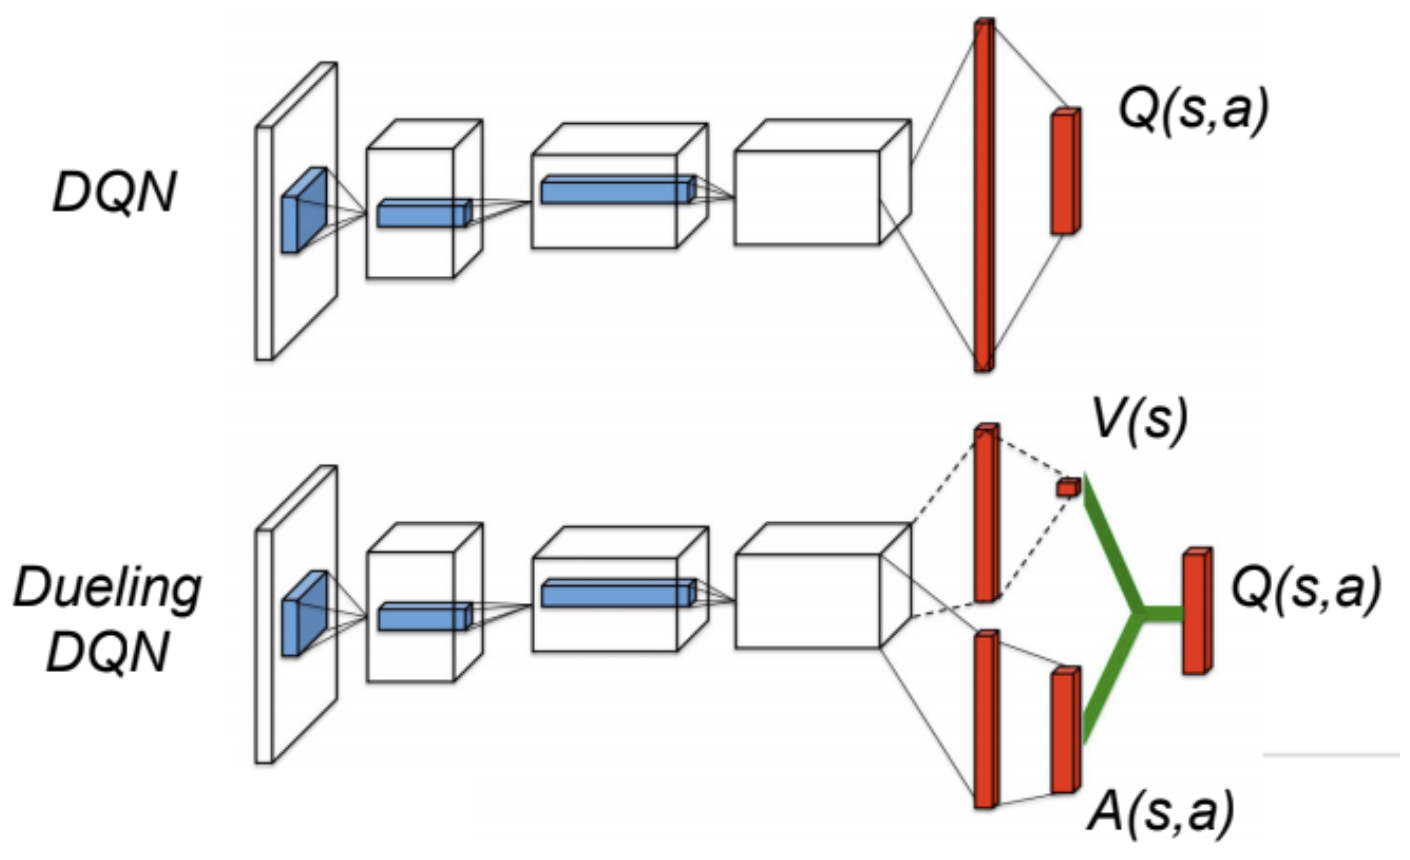
\includegraphics[width=\columnwidth]{dcn_and_ddcn.png}
\caption{Aufbau DCN und DDCN \cite{dcnddcn}}
\label{fig:dcnddcn}
\end{figure}

Anschließend wurde die Tauglichkeit des \textit{Duelling Deep-Q-Network-Algorithmus} (kurz: D-DQN) untersucht. Hierbei handelt es sich, wie der Name bereits andeutet, um eine Weiterentwicklung des vorherigen \textit{DQN-Algorithmus}: der zuvor erläuterten \textit{Q-Table} wird hierbei nun auch ein Wert hinzugefügt, welcher den aktuellen Zustand bewertet (s.h. Abb. \ref{fig:dcnddcn}). 

Es stellte sich allerdings auch hier nach zwei Stunden Training kein sichtbarer Lernerfolg ein, wodurch auch dieser im Rahmen dieser Studienarbeit ungeeignet ist.

\begin{figure}[hbt!]
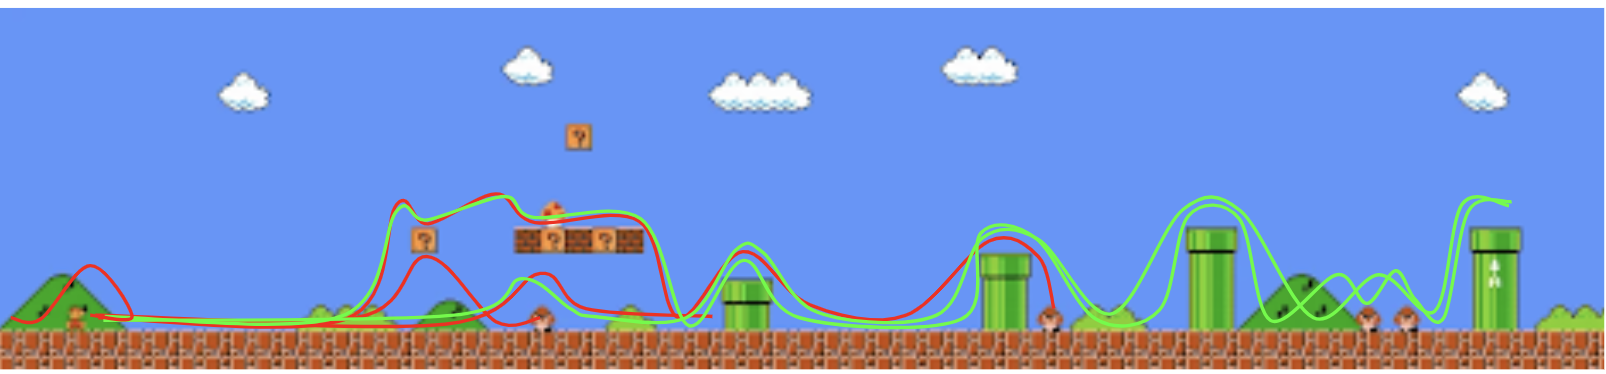
\includegraphics[width=\columnwidth]{smb_routes.png}
\caption{Mögliche Laufwege in SMB (Org.: \cite{smbroutes})}
\label{fig:smbroutes}
\end{figure}

Ursächlich für den geringen Lernerfolg ist hierbei die Komplexität des ursächlichen Problems bzw. der Aufgabe: Betrachtet man die Menge an Zuständen, so fällt auf, dass diese potentiell gegen unendlich läuft, ebenso ist es bei der Menge an möglichen Aktionen. 

Betrachtet man Abbildung \ref{fig:smbroutes} so sind ein paar Laufwege von Mario eingezeichnet. Mit grünen Linien sind die erfolgreichen Laufwege markiert, in rot hingegen sind erfolglose Laufwege markiert.

Genannte gegen unendlich laufende Menge an Zuständen entspricht in der Grafik jeden Punkt auf einer Linie, die innerhalb des SMB-Enviorments auch gerendert werden kann. Die ebenfalls gegen unendlich laufende Menge an Aktionen entspricht hierbei der Anzahl an zeichenbaren Laufwegen, welche den Regeln des SMB-Enviroments folgen. 

Diese beiden Mengen entsprechen den \textit{Input} und den \textit{Output} des Modells und definieren dadurch wichtige Eigenschaft des zur Lösung geeigneten Algorithmus.

Dies in Kombination mit der Tatsache des Trainierens auf einem einzigen Thread erklärt die Überlegenheit des nachfolgenden Algorithmus. \cite{dqnmedium}, \cite{ddqndatascience}

\subsection{A3C-Ansatz}
\label{a3c}

Ein \textit{Reinforcement-Learning-Algorithmus}, der hingegen besser Performance bei dieser Komplexität verspricht ist der \textit{Asynchronous-Advantage-Actor-Critic-Algorithmus} (kurz: A3C).

\begin{figure}[hbt!]
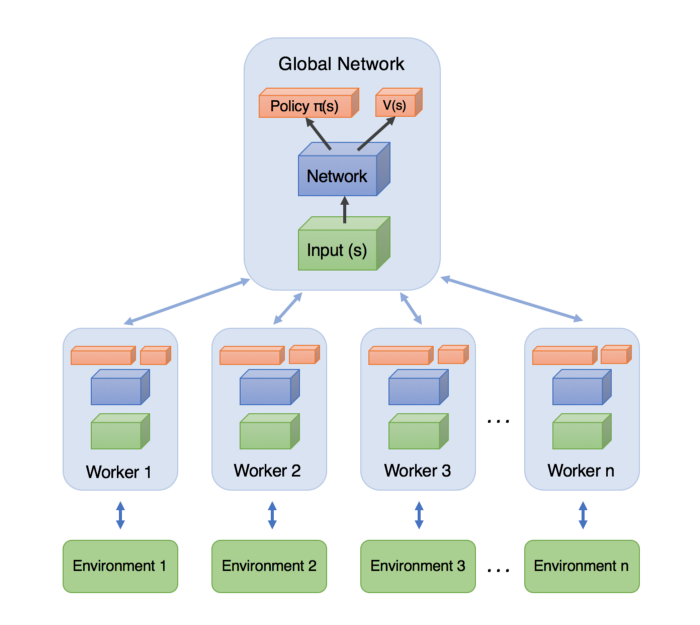
\includegraphics[width=\columnwidth]{a3c.png}
\caption{Aufbau A3C \cite{a3cmedium}}
\label{fig:a3c}
\end{figure}

Im Gegensatz zur den vorher genannten Algorithmen wird hier keine \textit{Q-Table} erzeugt. Stattdessen wird unter Berücksichtigung einer geschätzten Bewertung des aktuellen Zustandes vom sog. \textit{Critic} (deutsch: Kritiker), eine Aktion ausgeführt vom sog. \textit{Actor} (deutsch: Akteur). Der \textit{Actor} und der \textit{Critic} werden hierbei als separate Neuronale-Netzwerke definiert, die den exakt gleichen Input erhalten müssen.

Die Idee des A3C-Algorithmus lässt sich also mit folgender Metapher gut erklären.
\begin{quote}
Let['s] imagine a small mischievous child (actor) [which] is discovering the amazing world around him, while his dad (critic) oversees him, to make sure that he does not do anything dangerous. Whenever the kid does anything good, his dad will praise and encourage him to repeat that action in the future. And of course, when the kid does anything harmful, he will get [a] warning from his dad. The more the kid interacts [with] the world, and takes different actions, the more feedback, both positive and negative, he gets from his dad. The goal of the kid is, to collect as many positive feedback as possible from his dad, while the goal of the dad is to evaluate his son's action better. In other word, we have a win-win relationship between the kid and his dad, or equivalently between actor and critic.\cite{nguyen}
\end{quote}

Dieser Ansatz wird durch parallel agierenden Modelle erweitert, welche wiederum regelmäßig (in der Regel abhängig von der definierten Batchgröße) ein gemeinsames Model (sog. \textit{globales Model}) aufbauen bzw. trainieren und sich auf dessen Lernstand selbst aktuell halten.

Mit diesem Algorithmus kam es bereits nach wenigen Minuten zu einem sichtbaren Lernerfolg, nach 2 Stunden wurde so das Lernziel des Experiment, das Abschließen eines Level, bereits erreicht. Es zeichnete sich also ab, dass dieser Algorithmus bestens geeignet ist für das eigentliche Experiment. \cite{a3cchris}, \cite{a3cmedium}

\section{Enviroment}
Wie bereits erwähnt kommt in diesem Experiment ein SMB-Enviroment zum Einsatz (vgl. \ref{smbgym}), nachfolgend wird die Konfiguration und der Einsatz dieses \-SMB-\-Env\-iro\-ment genauer betrachtet.

\subsection{Konfiguration}
\label{smbconfig}
Auf Basis von Vorab-Experimenten wurde sich für die Standard Render-Version entschieden, welche eine minimal schlechtere Lernperformance - in diesem Fall das erstmalige Erreichen des Zieles - als die anderen bereitgestellten grafisch reduzierten Render-Versionen aufwies.

Ausgehend von den selben Vorab-Ergebnissen wurde sich für eine leicht reduzierte Eingabemenge (im '\textit{Super Mario Bros for OpenAI Gym}' \cite{gym-smb} 'Complex' genannt) entschieden. Diese beinhaltet im wesentlichen neben einer leeren Eingabemenge auch  Kombinationen aus den Nach-Links- oder Nach-Rechts-Tasten mit der A- oder bzw. und B-Taste des \textit{NES}-Controllers. Die  weiteren reduzierten Eingabekombination hatten einen zustandsabhängigen Einfluss auf das Ergebnis, wodurch einige Level des Enviroments merklich schneller andere merklich langsamer erlernt wurden.

\subsection{Weitere Modifikationen}
Mittels  \textit{Wrapper-Pattern} wurde der \textit{Output} des ursprünglichen Enviorments modifiziert. Nachfolgend werden diese Modifikationen von innen nach außen kurz erläutert.

\begin{figure}[hbt!]
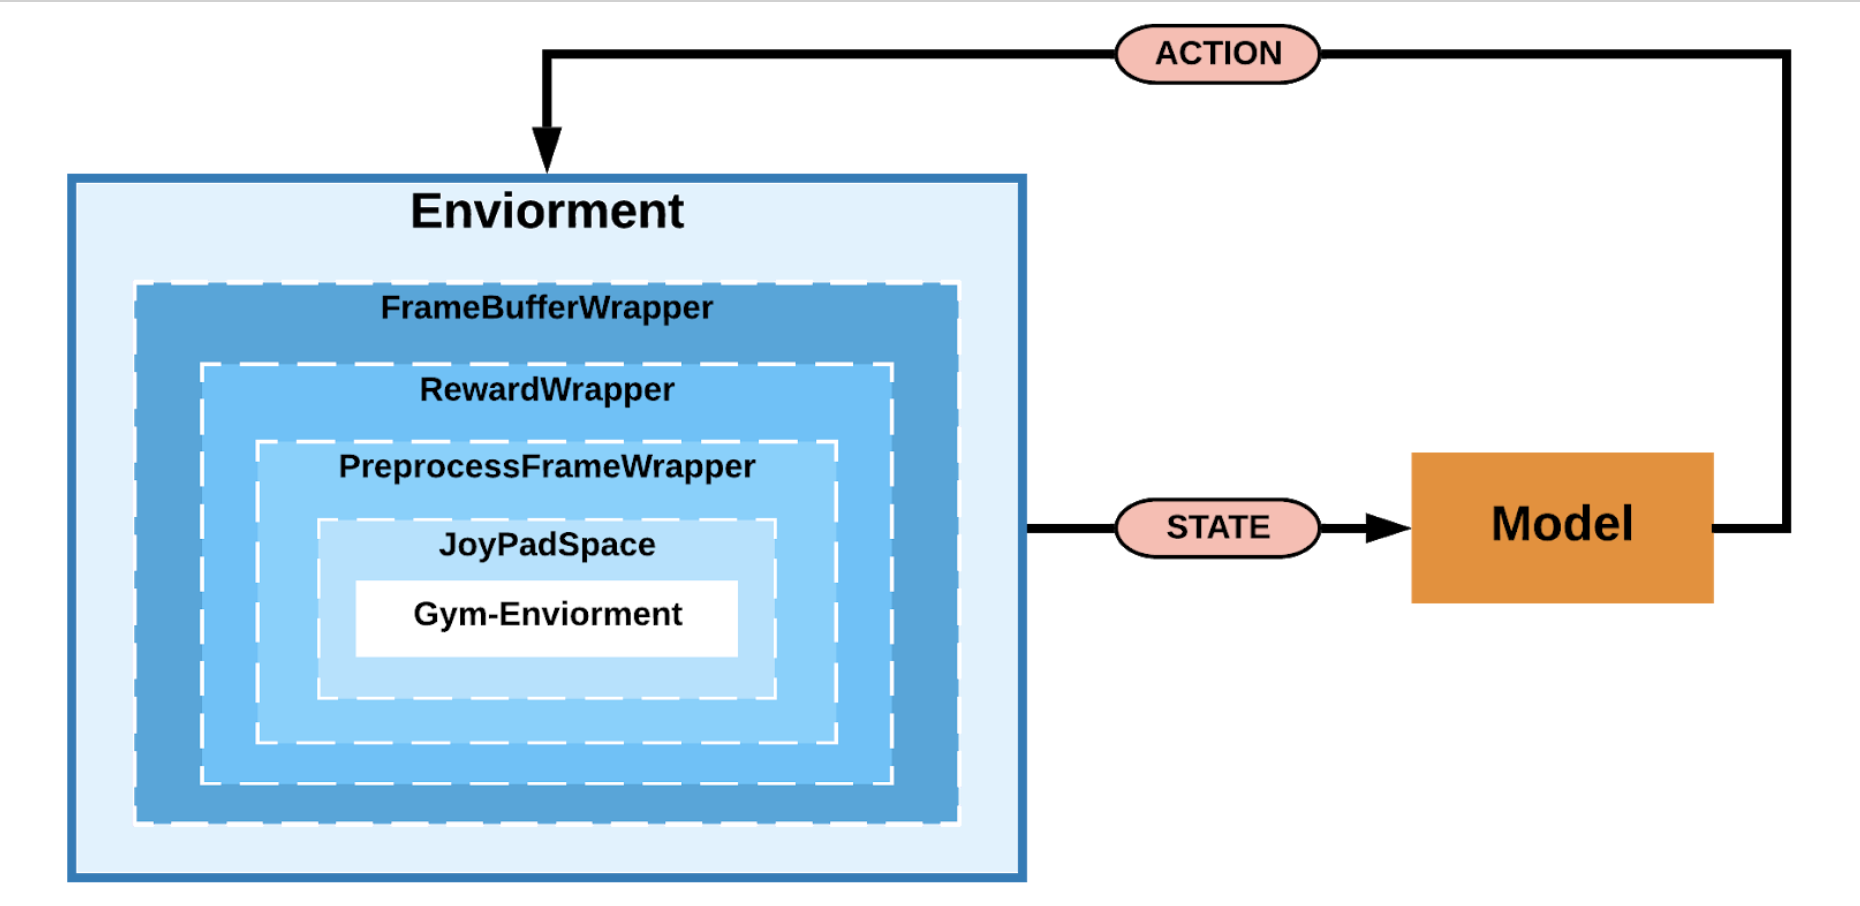
\includegraphics[width=\columnwidth]{env_context.png}
\caption{Schematischer Kontext des konkret implementierten Enviorments}
\end{figure}

\subsubsection{JoypadSpace}\hfill \break
Der \textit{JoypadSpace-Wrapper} ist eine von \textit{OpenAI} zur Verfügung gestellte Implementation des \textit{OneHot-Encodings} für das \textit{NES}.

\subsubsection{PreprocessFrameWrapper}\hfill \break
Der \textit{PreprocessFrameWrapper} vorverarbeitet den ursprünglichen berechneten Frame (vgl. \ref{preprocessing}).

\subsubsection{RewardWrapper}\hfill \break
Der \textit{RewardWrapper} überschreibt den ursprünglich berechneten Rewardwert (vgl. \ref{reward}).

\subsubsection{FrameBufferWrapper}\hfill \break
Der \textit{FrameBufferWrapper} fasst einige berechnete Frames in ein Array zusammen, um so dem Model die Chance zu bieten Bewegungen zu erkennen.

\subsection{Preprocessing}
\label{preprocessing}
Das \textit{Preprocessing} dient zur Vorverarbeitung des Frames. Dadurch soll das Bild so angepasst werden, dass das zutrainierende Model damit bestmöglich rechnen kann. In der konkreten Implementation kann dieser Schritt in wiederum vier Teilschritte unterteilt werden, die nachfolgend kurz begründet werden.

\begin{figure}[hbt!]
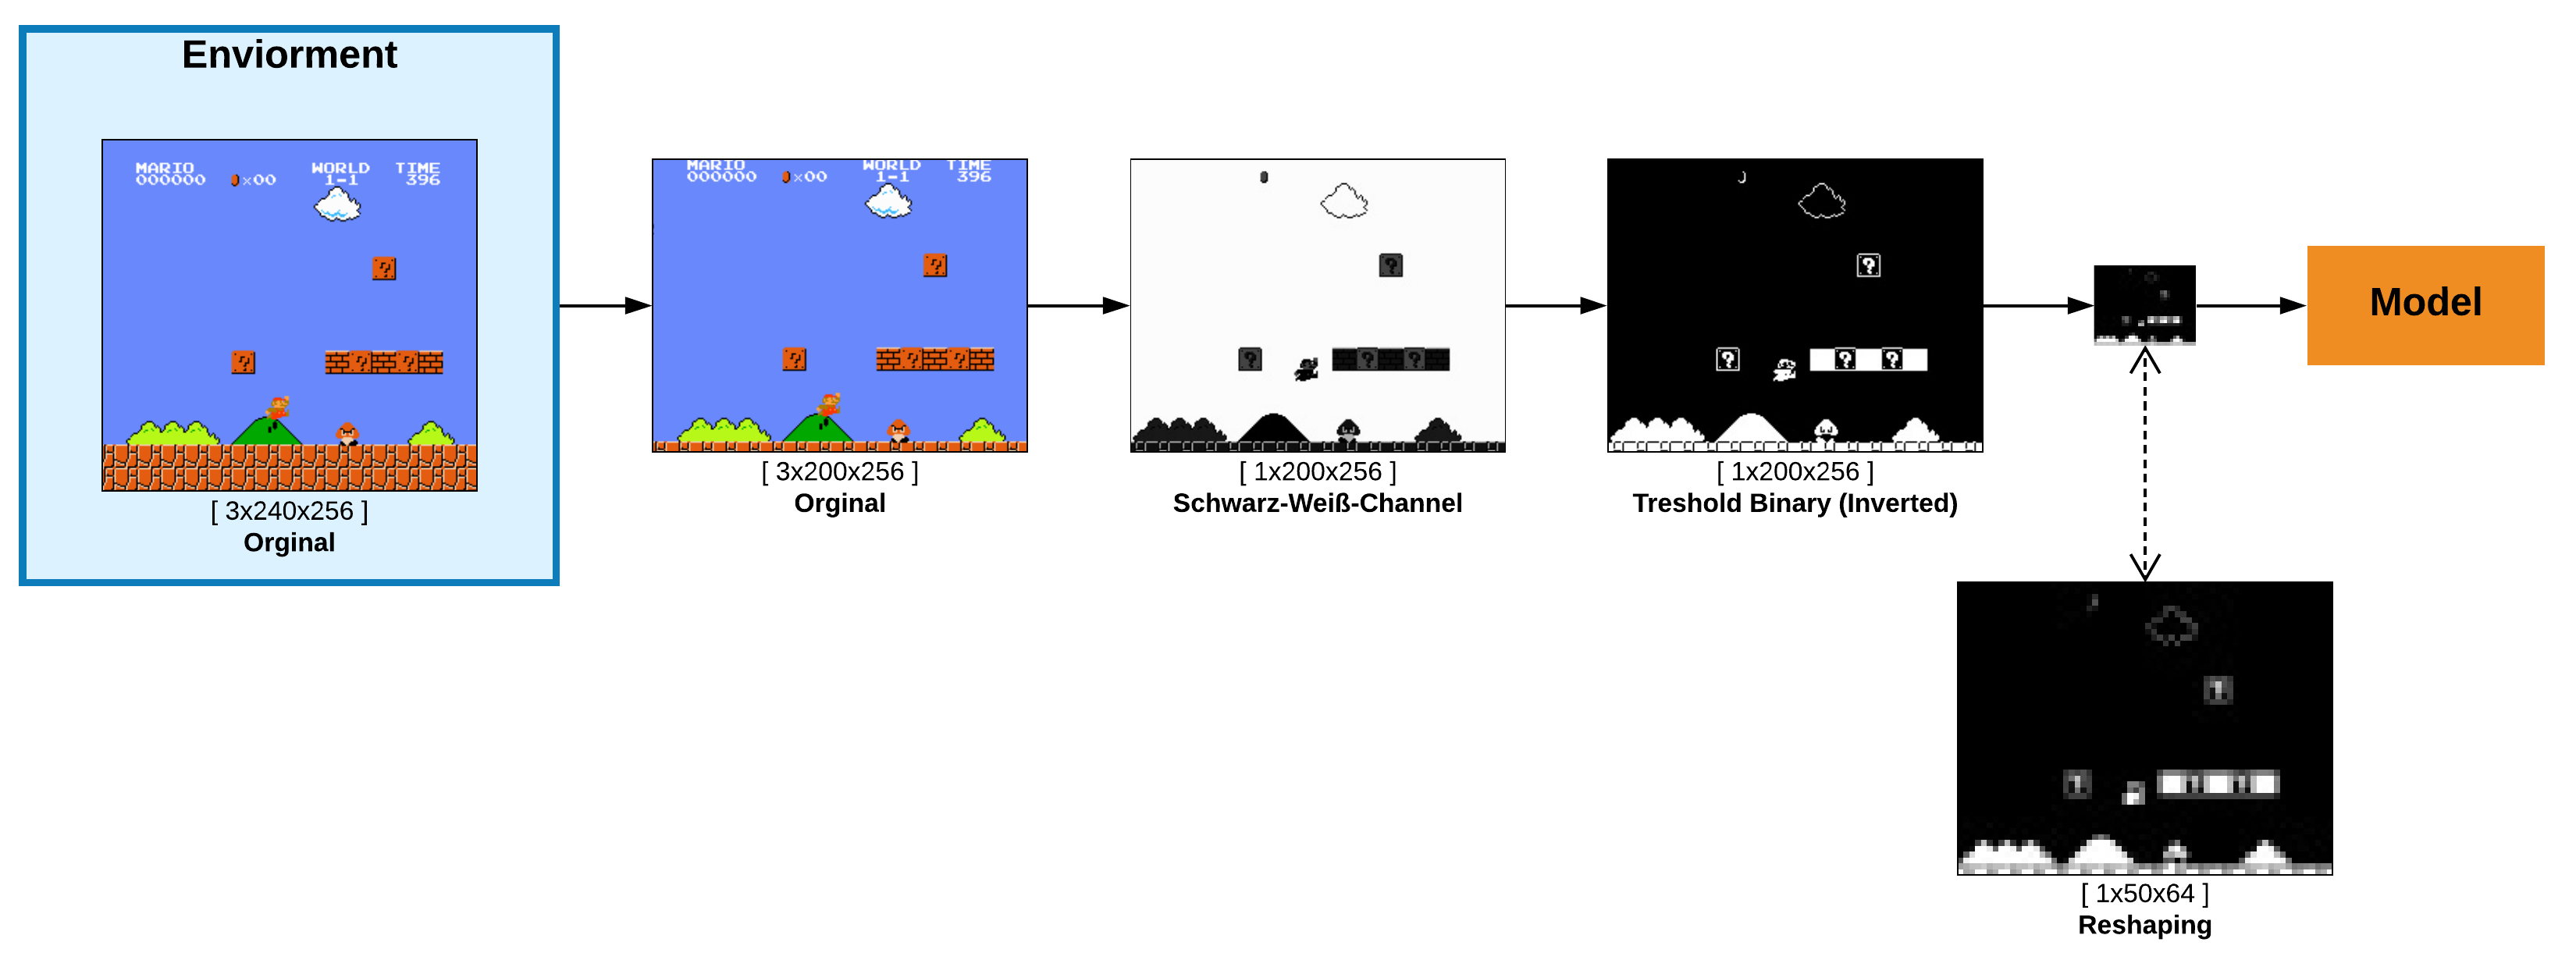
\includegraphics[angle=90,scale=0.08]{preprocessing.png}
\caption{Schematische Preprocessing}
\end{figure}

\subsubsection{Zuschneiden}\hfill \break
Zuerst wird der originale 240x256 Pixel große Frame auf 200x256 Pixel verkleinert. Konkret werden einige Pixel oben und unten weggeschnitten, welche (fast) keine Relevanz für den Spielverlauf haben.

\subsubsection{Schwarz-Weiß}\hfill \break
Im nächsten Schritt wird der Frame zu einem verlustfreien Schwarz-Weiß-Bild vereinfacht.

\subsubsection{Schwarz-Oder-Weiß}\hfill \break
Anschließend wird der Frame mittels \textit{Binary-Treshhold} zu Schwarz- oder Weißenfarbtönen vereinfacht. Damit diese sich auch optisch von dem vorherigen Schritt leicht unterscheiden lassen, werden hierbei die Farben invertiert.

\subsubsection{Verkleinern}\hfill \break
Abschließend wird das Bild im korrekten Seitenverhältnis verkleinert. Dies hat u.a. Einfluss darauf wie viel Speicher das Model in allen Ebenen benötigt und wurde im Rahmen des Experimentes auf 50x64 Pixel gesetzt (vgl. \ref{hardware}) - dies entspricht nahezu der minimalen informationsverlustbehafteten Verkleinerung des Bildes, die im Rahmen diverser Experimente festgelegt worden ist.

\subsection{Reward}
\label{reward}
Der \textit{Reward} definiert das mathematisch entstehende Verständnis des Modells über das Enviorment. Hierfür gibt es in der Regel zwei unterschiedliche Ansätze, wie dieser \textit{Reward} vergeben werden kann: Per \textit{Sparse Reward} oder mittels \textit{Reward Shaping}. Beim sog. \textit{Sparse Reward} wird der \textit{Reward} nur beim Erreichen wesentlicher Ziele vergeben. Beim \textit{Reward Shaping}, welches für das Experiment gewählt wurde, wird hingegen durch kontinuierliches Vergeben des \textit{Reward} das mathematische Verständnis des Modells sehr stark beeinflusst, wodurch eine starke Abhängigkeit zwischen der Qualität der \textit{Reward-Funktion} und dem Lernergebnisses ensteht.

Im der konkreten Implementation besteht der \textit{Reward} aus 4 Werten, die nach einer Addition in einen geringeren Wertebereich verschoben werden: 

\begin{equation}
F_{Reward}=(\Delta X+\Delta Zeit+R_{Ziel}+R_{Leben})\ /\ 10
\end{equation}\hfill \break

Dem Delta der zurückgelegten Strecke addiert mit der verstrichenen Zeit, zusätzlich den fest definierten Belohnungswerten für das erreichen des Zieles bzw. für das verlieren eines Lebens. Diese Variablen lassen sich wie folgt definieren:

\begin{equation}
\Delta X = X(n+1) - X(n)
\end{equation}
\begin{equation}
\Delta Zeit = T(n+1) - T(n)
\end{equation}
\begin{equation}
R_{Ziel} = 45\ if\ goal\ achieved\ else\ 0
\end{equation}
\begin{equation}
R_{Leben} = -45\  if\ life\ lost\ else\ 0
\end{equation}\hfill \break

Ziel des Modells für die \textit{Reward-Funktion} ist es also eine möglichst große Distanz in geringer Zeit zu erreichen, bei denen im bestenfalls das Ziel erreicht wird und idealerweise kein Leben verloren wird.

Experimente mit weiteren Faktoren wie etwa einer Belohnung für das Sammeln von Münzen oder dem Verhindern des 'Stehenbleibens' hatten meist negative Auswirkungen auf das eigentliche Hauptziel.

\section{Netzwerk-Architektur}
Die zugrundeliegende Netzwerk-Architektur für den \textit{A3C-Algorithmus} erfordert zwei separate Netzwerke (\textit{Actor} und \textit{Critc}), die wiederum sich den selben \textit{Input} teilen. Dieser \textit{Input} entsteht durch visuelle Verarbeitung mittels \textit{Convolutional-Netzwerkes} (kurz: CNN) und anschließend durch rückgekoppelte Verarbeitung mittels \textit{Rekurrentem-Netzwerkes} (kurz: RNN) mit dem Ziel der reihenfolgeabhängigen Verarbeitung. Auf all diese Bestandteile des implementierten Neuronalen Netzwerkes wird nachfolgend eingegangen (vgl. Abb. \ref{fig:KontextModel}).

\subsection{Convolutional-Netzwerk}
Wie erwähnt dient das \textit{CNN} dazu grafische nicht näher definierte Muster innerhalb des Frames zu deuten. Es wurden hierbei zwei unterschiedliche Architekturen definiert, die nachfolgend kurz erklärt werden. Beide Ansätze hatten zum Ziel die \textit{Tensorgröße} zu minimieren, um dadurch die limitierte Hardware (vgl. \ref{hardware}) bestmöglichst auszunutzen.

\subsubsection{Naive CNN}\hfill \break
Bei dem Naiven Ansatz des \textit{CNN} wird ein initial 320 Channel großer Tensor konstant um 80 Channel, also ursprünglich um 25\%, verkleinert. Hintergrund hierfür ist, neben dem Ziel den Tensor klein zuhalten, dass mehrere Frame-Features zu einem einzigen Signal inkrementell zusammengefasst werden sollen. Als Kernelgröße wurde 3x3 gewählt, bei einem Stride von 2, welcher u.a. den Tensor konstant reduziert.

Während der Entwicklungsphase gab es keine wesentlichen Unterschiede bei ähnlich hoher Start-Channel-Anzahl und Channel-Reduktionsfaktor, weshalb die Größen so gewählt wurden, dass der verfügbare Arbeitsspeicher voll ausgelastet wurde.

\begin{figure}[hbt!]
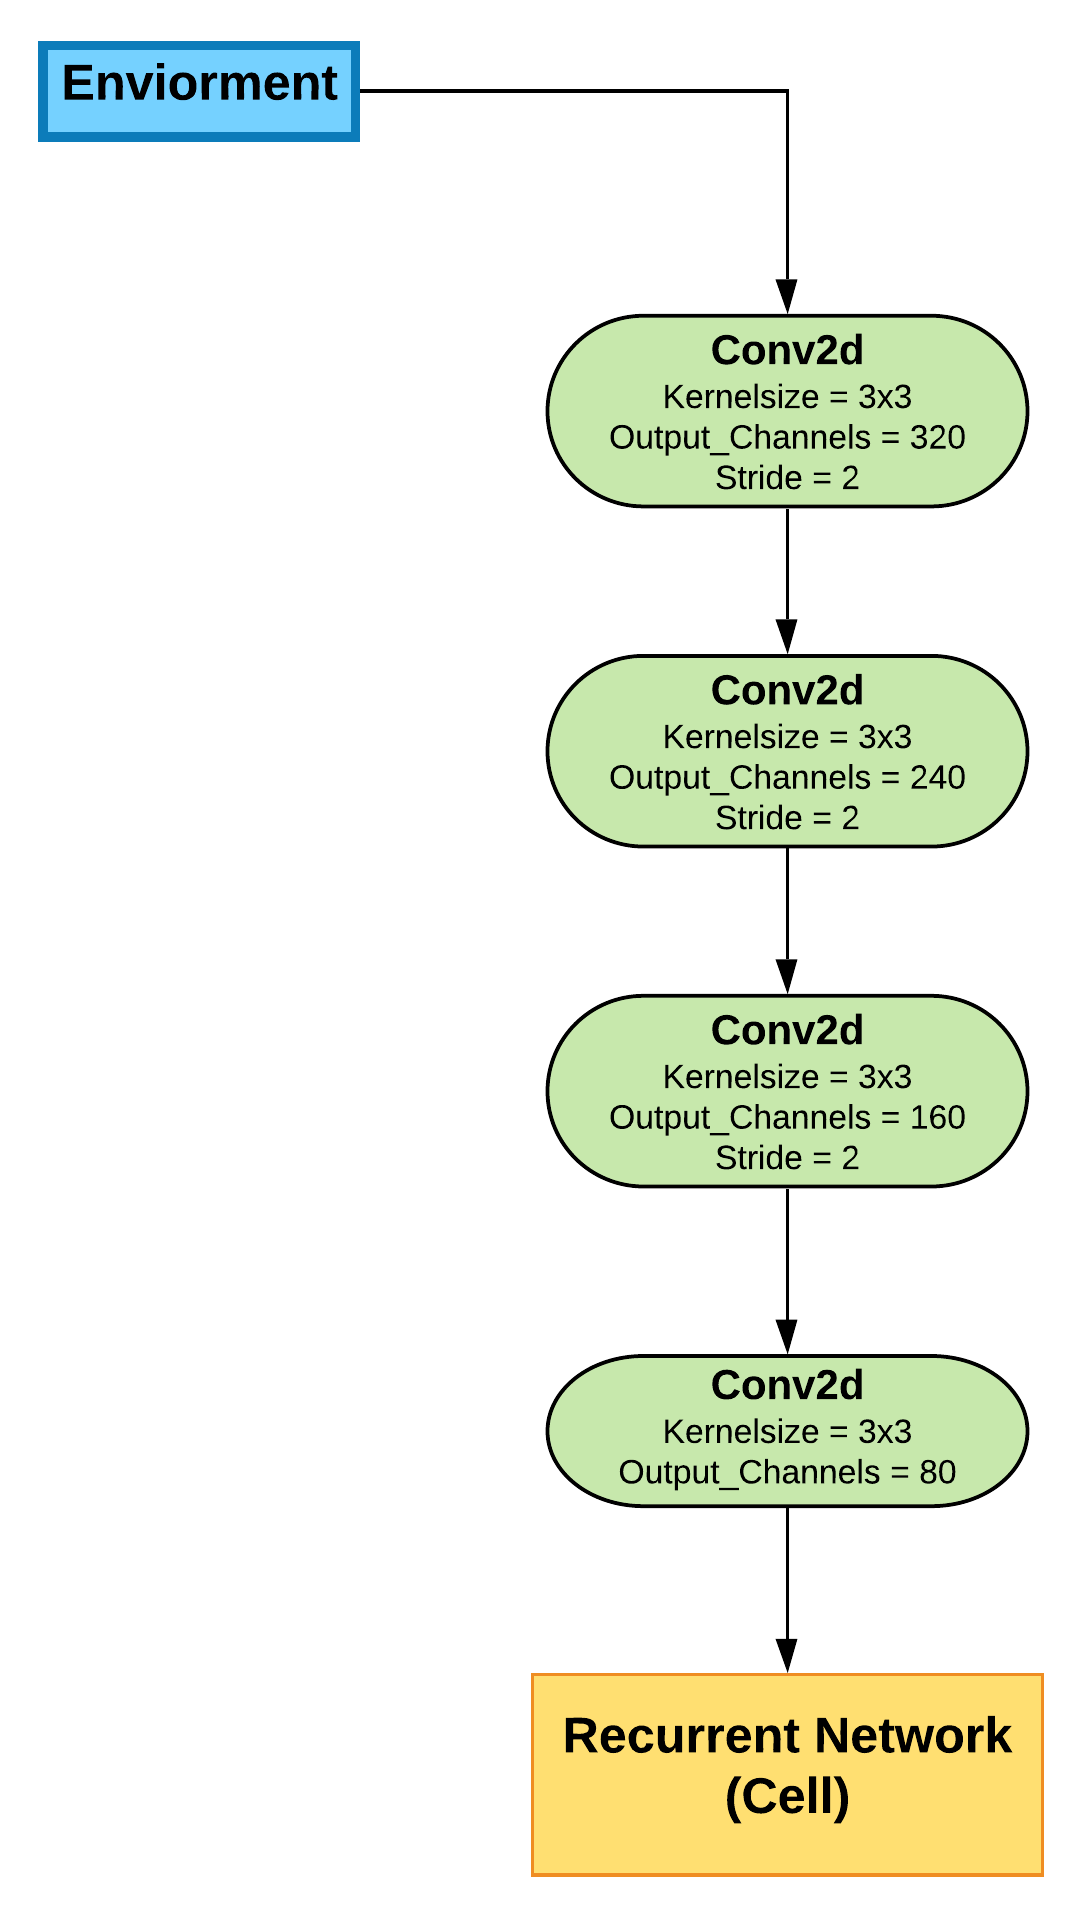
\includegraphics[height=\columnwidth]{Netzwerk_Architektur_cn.png}
\caption{Naive CNN-Architektur}
\end{figure}

\subsubsection{Deep(ish)-CNN}\hfill \break
Ein weiterer Ansatz für den \textit{CNN}-Teil ist inspiriert von den \textit{GoogLeNet}-Blöcken \cite{he2015deep}. Im Gegensatz zu den vorherigen \textit{CNN}-Ansatz kamen hier nach jedem \textit{CNN}-Layer eine \textit{ReLU}-Aktivierungsfunktion zum Einsatz. Wie auch in dem naiven \textit{CNN}-Ansatz wird hier mittels Stride die Tensorgröße effektiv reduziert.

Abweichend zu \textit{GoogLeNet} wurden hier im zweiten Branch drei 3x3 große Kernel und im dritten Branch zwei 5x5 große Kernel verwendet. Eine Reduktion der Rechenleistung durch das Ersetzen der 5x5 Kernel mittels zwei 3x3 Kernel ist hierbei aufgrund der Strides nicht möglich. Die Channelanzahl der einzelnen Branches wird unterschiedlich stark auf 32 reduziert, wodurch im letzten Verknüpfungschritt 128 Channel erreicht werden.

\begin{figure}[hbt!]
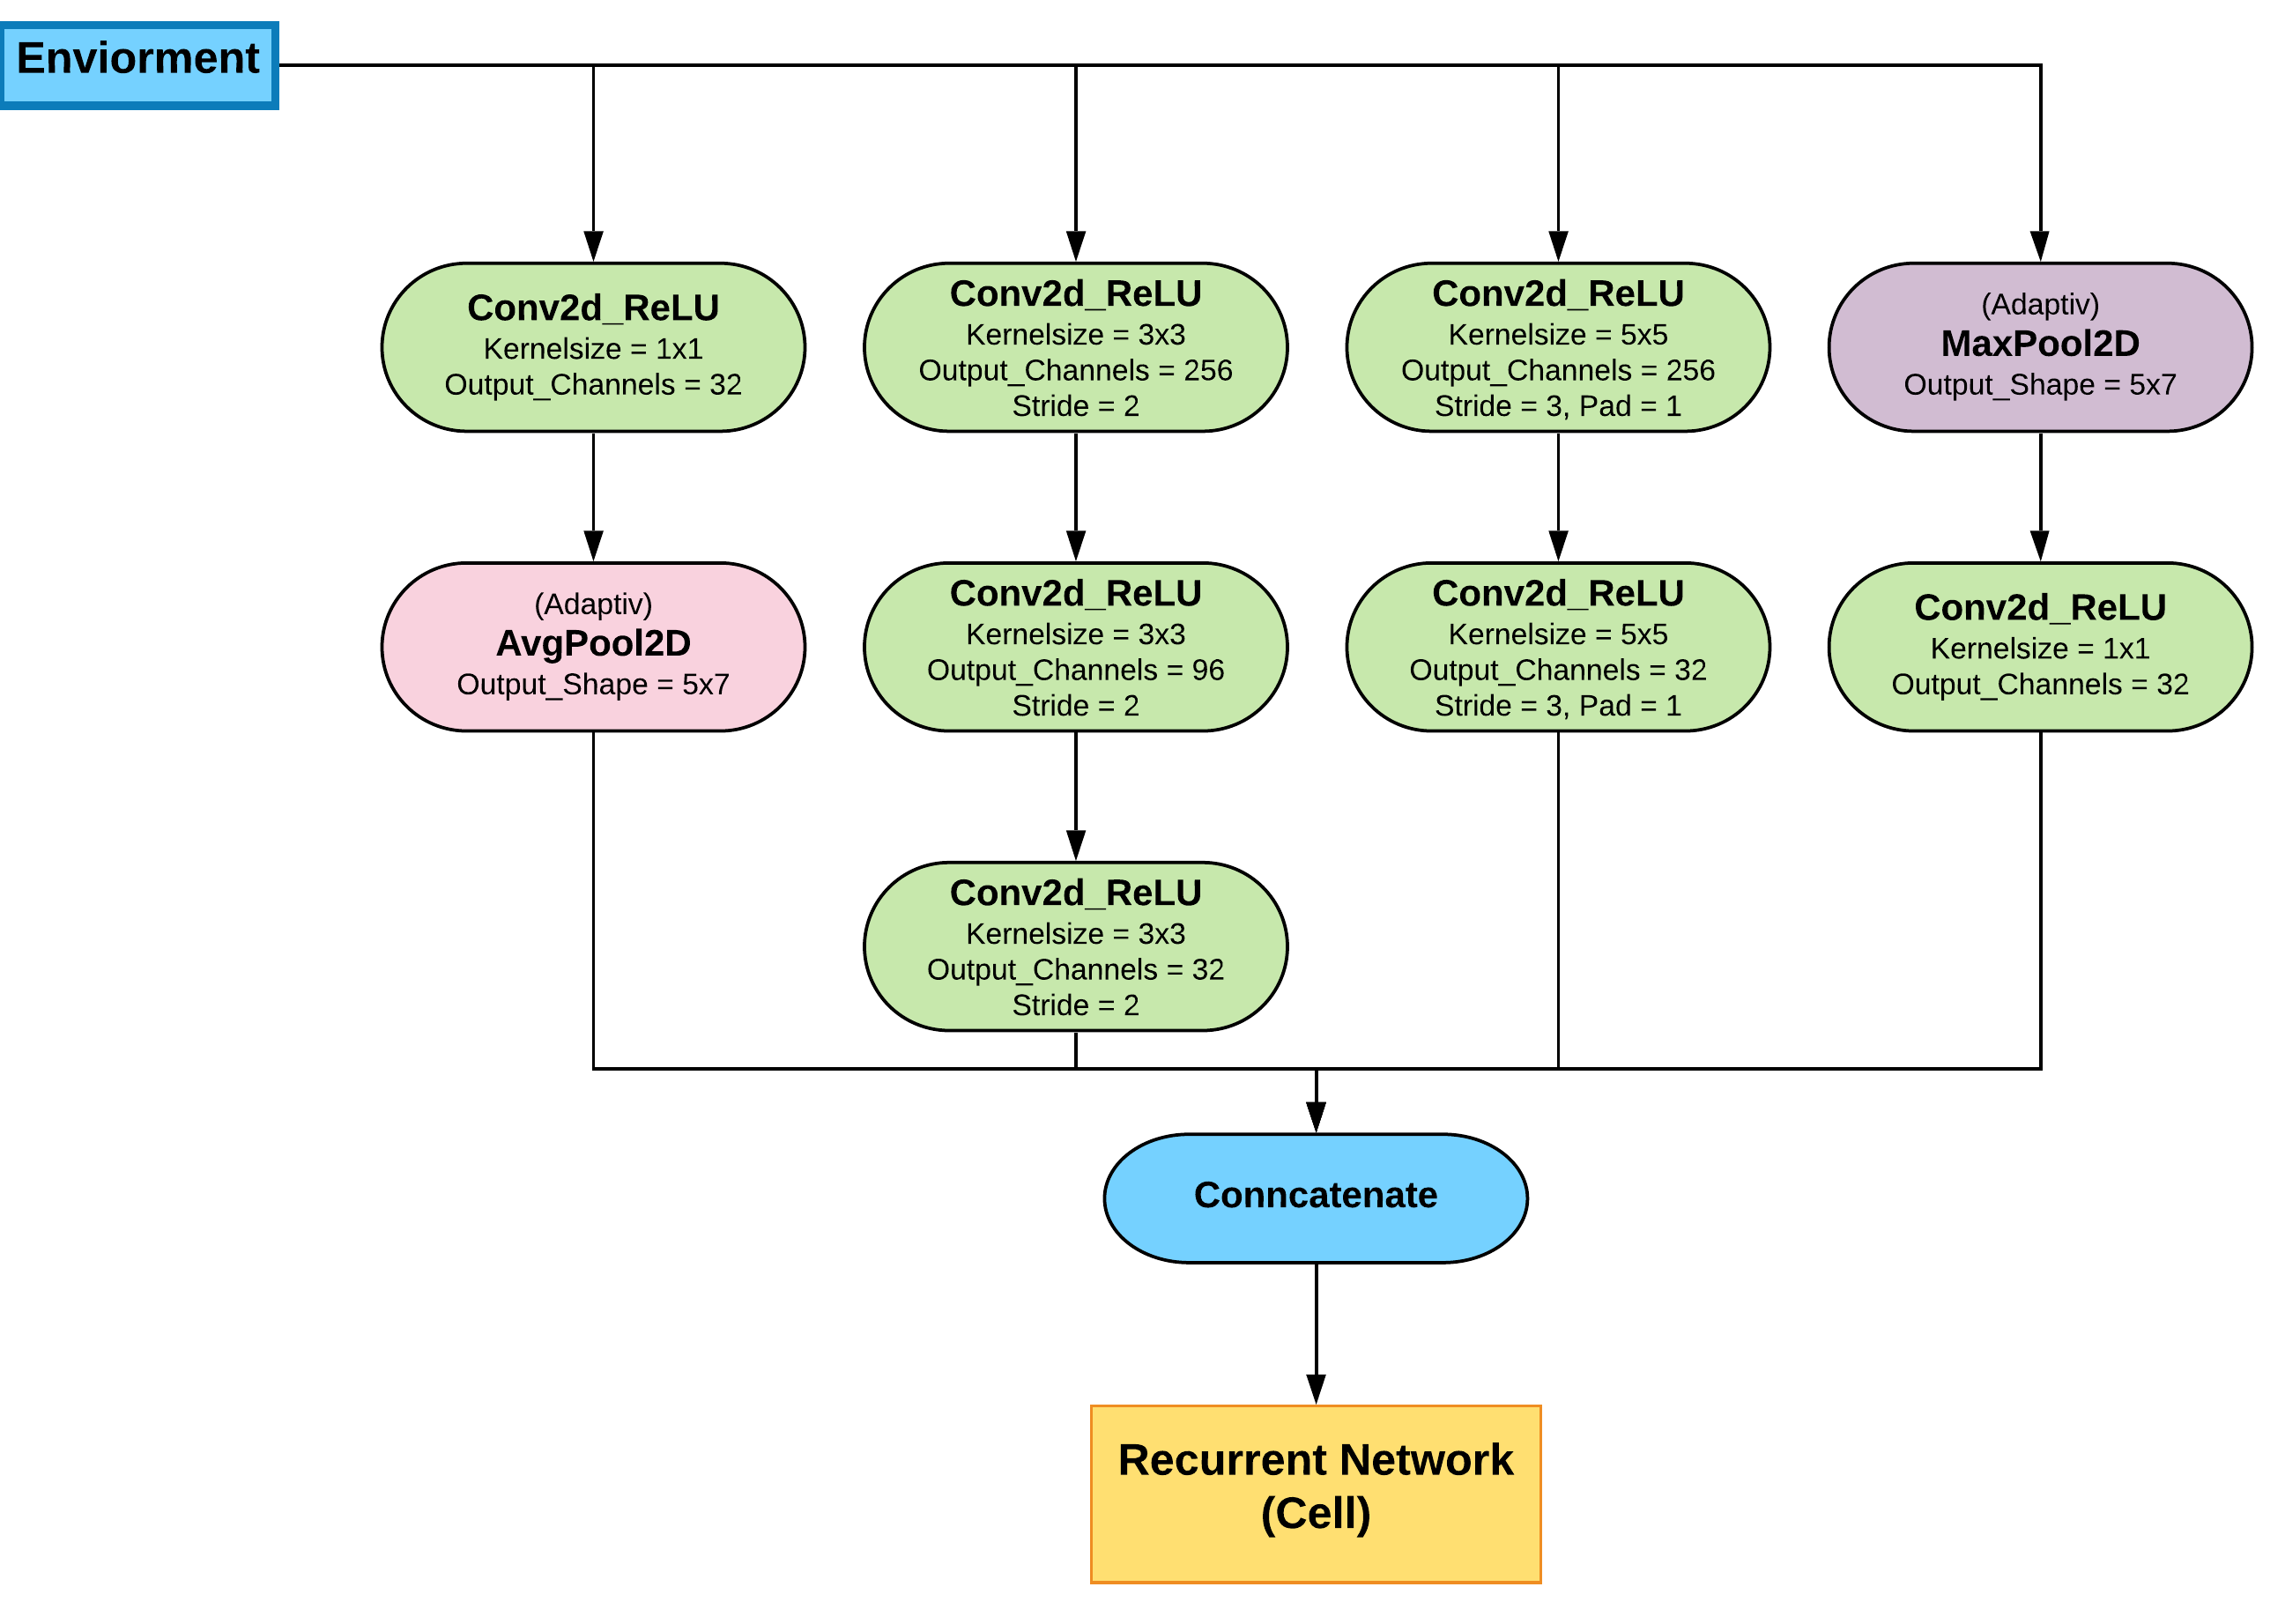
\includegraphics[angle=90,height=\columnwidth]{Netzwerk_Architektur_dcn.png}
\caption{Deep(ish)-CNN-Architektur}
\end{figure}
Die wesentlichen Abweichungen hinsichtlich der Kernelgröße und -anzahl sind hauptsächlich experimentell zu erklären. Geringe Änderungen hierbei hatten meist eine längeren Lernzeit für ähnliche Lernergebnisse zufolge. Die Anzahl an Channels ist ähnlich wie bei dem Naiven \textit{CNN}-Ansatz mit der Hardware-Ausnutzung begründet (vgl. \ref{hardware}).

\subsection{Rekurrent-Netzwerk}
Hinsichtlich des Rekurrent-Netzwerk stellte es sich als problematisch heraus, dass zu dem Zeitpunkt, an dem ein \textit{CNN-Output} generiert wurde das Training noch nicht abgeschlossen wurde, weshalb kein allgemeines \textit{RNN} implementiert wurde. Stattdessen wurde eine Zelle implementiert, die als Teilinput den Output der selben Zelle zu dem vorherigen Schritt des Enviorments erhält.

Da der \textit{RNN}-Teil für das absolvieren SMB ähnlicher Enviormente eine herausragende Rolle spielt, wurde die Channelanzahl innerhalb des kompletten Netzwerk maximiert. Da dies allerdings dazu führt, das bei der zur Verfügung stehenden limitierten Hardware, ein stark ansteigender Arbeitsspeicherverbrauch entsteht, wodurch diverse Abhängigkeiten innerhalb des Netzwerks und dem Enviroment ensteht, fehlten zum Zeitpunkt des Experimentes weitere Untersuchungen hinsichtlich der optimalen Werte.

\subsubsection{LSTM-RNN}\hfill \break
Ein Ansatz für das \textit{RNN} war die Verwendung der \textit{LSTM-Zelle}. Hier wird im Vergleich zum folgenden \textit{GRU}-Ansatz zusätzlich der \textit{Hidden-State} ebenfalls pro Berechnungsschritt übergeben. (Die Input-Channelanzahl ist Abhängig von der Output-Channelanzahl des \textit{CNN}-Teils.)

\begin{figure}[hbt!]
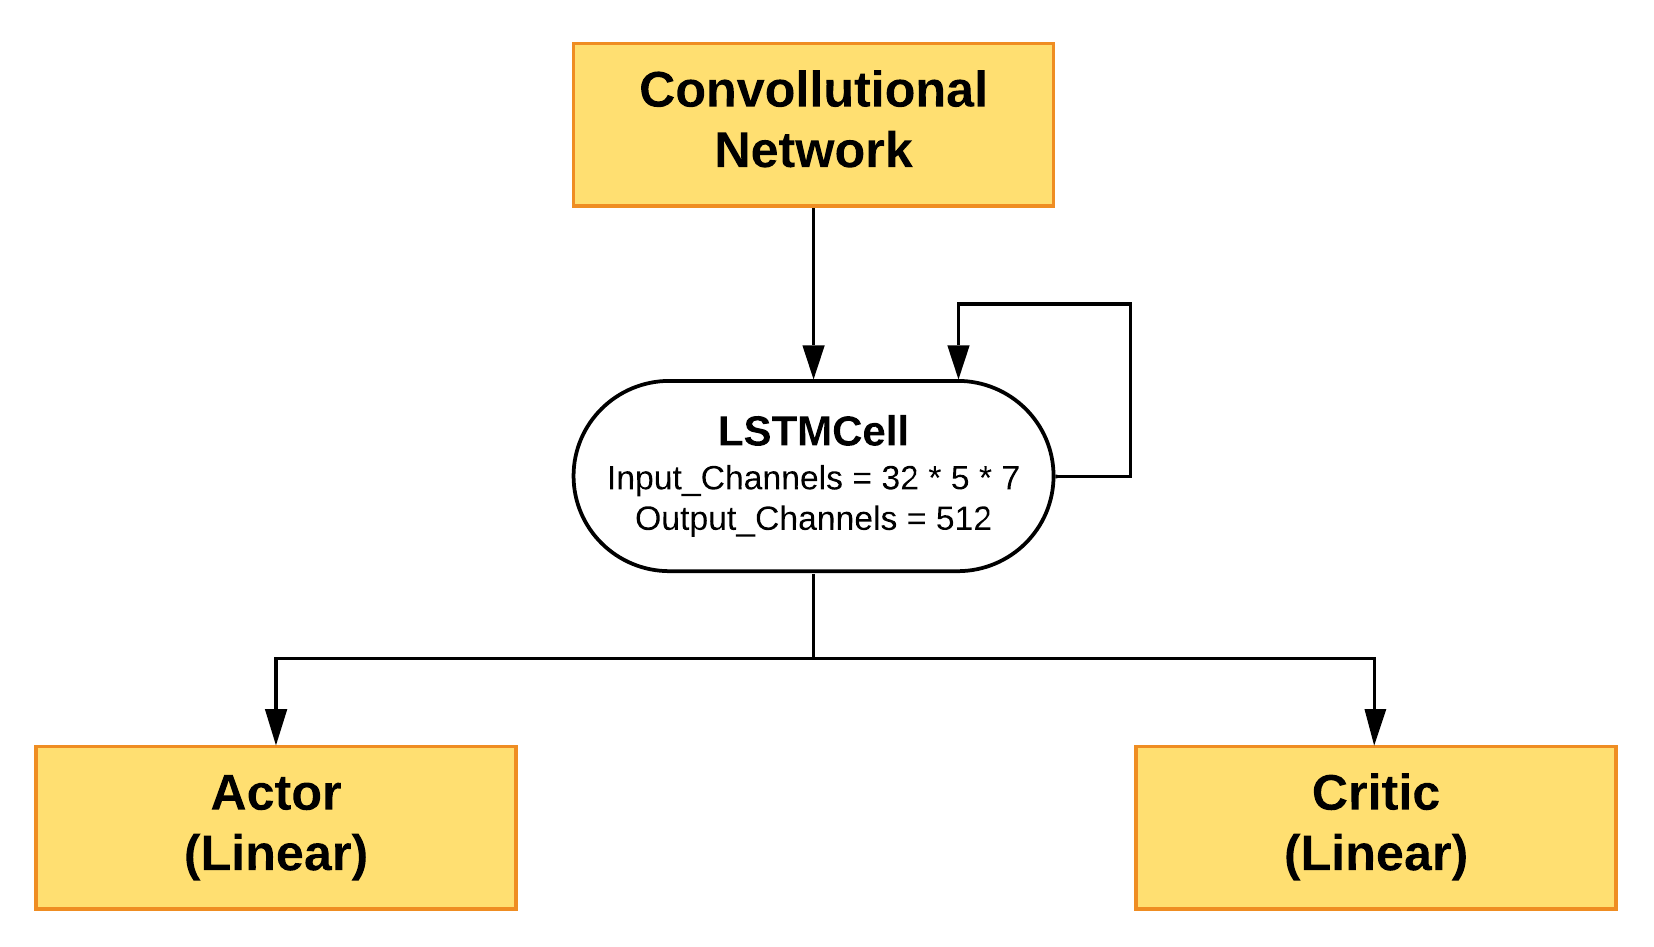
\includegraphics[scale=0.125]{Netzwerk_Architektur_lstm.png}
\caption{LSTM-Architektur}
\end{figure}

\subsubsection{GRU-RNN}\hfill \break

Ähnlich wie die \textit{LSTM-RNN}-Variante wurde die \textit{GRU}-Zelle verwendet. (Die Input-Channelanzahl ist Abhängig von der Output-Channelanzahl des \textit{CNN}-Teils.)

\begin{figure}[hbt!]
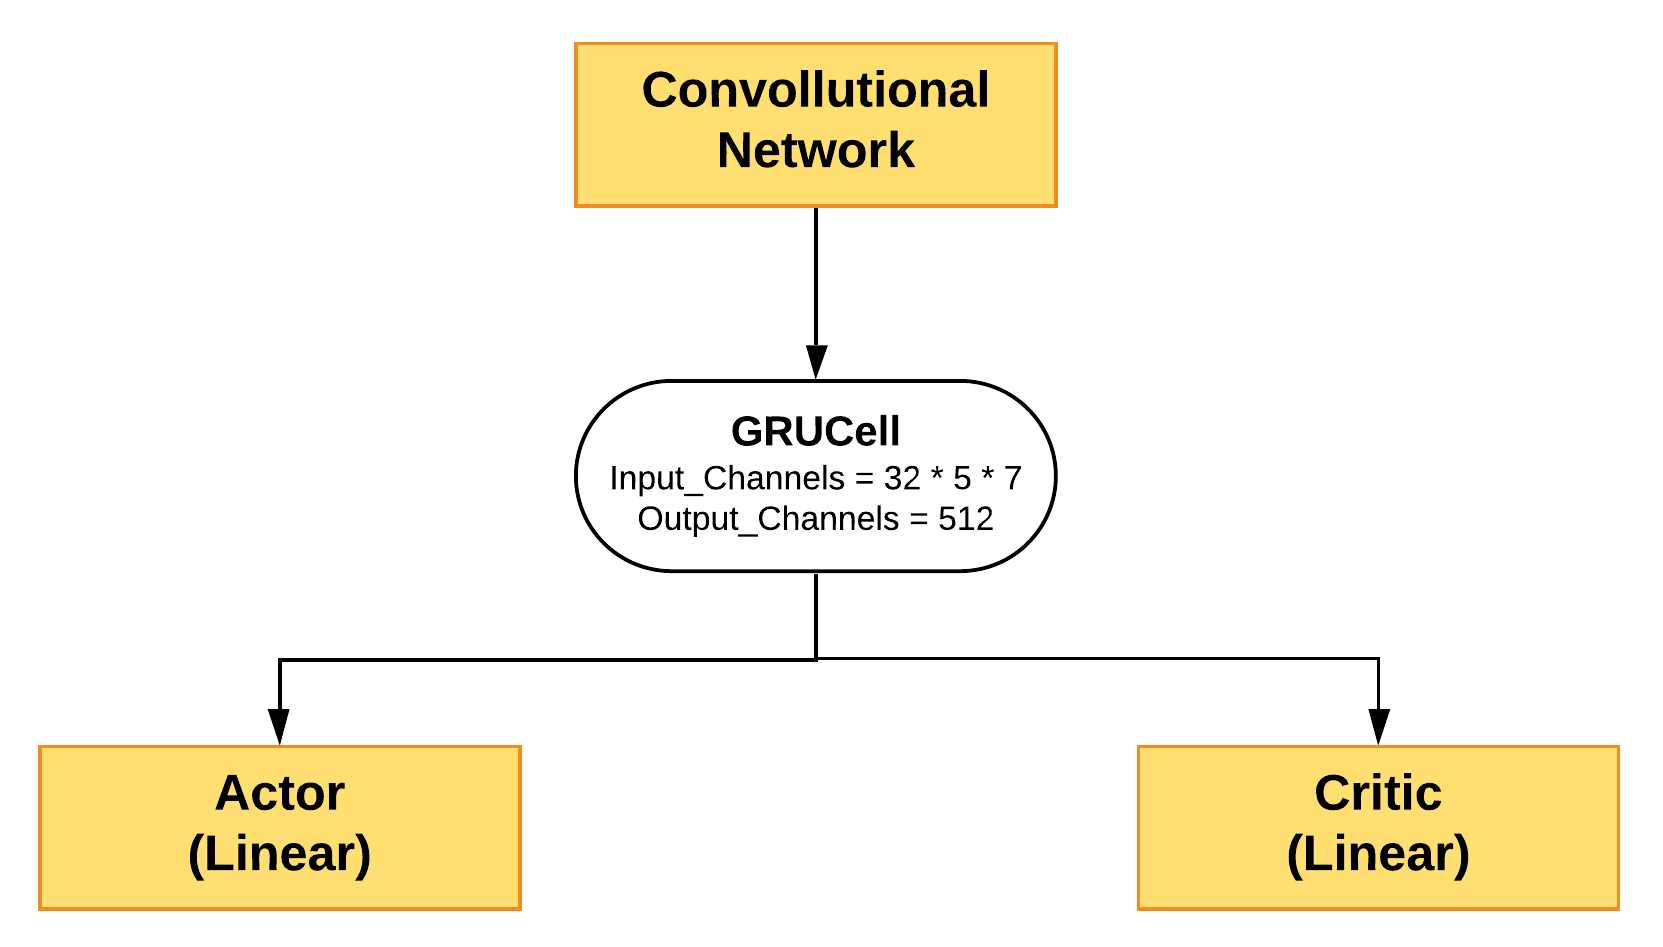
\includegraphics[scale=0.125]{Netzwerk_Architektur_gru.png}
\caption{GRU-Architektur}
\end{figure}

\subsection{Actor und Critic}
Der \textit{Actor-} und \textit{Ciritc-}Teil des neuronalen Netzwerkes spielt eine entscheidende Rolle für das Bestimmen der Aktionen. Als \textit{LinearerLayer} implementiert unterscheiden sich die beiden hauptsächlich im Output: Der \textit{Kritiker} berechnet einen einzigen Wert - die Bewertung des aktuellen Zustandes (vgl. \ref{fig:a3c}).

Der \textit{Akteur-Output} hingegen entspricht der Anzahl der verfügbaren Aktionen (vgl. \ref{smbconfig} und beinhaltet die Wahrscheinlichkeit das diese die bestmöglichste Aktion ist. Diese wird im weiteren Verlauf nach der wahrscheinlichsten Aktion gefiltert und zurück zu einer, für das Enviorment verständlichen Aktion, umgewandelt.

\subsection{Loss-Funktion}
Damit sich die zuvor aufgeführten \textit{Linearen-Layers} während des Trainings unterschiedlich entwickeln, werden diese in der Verlustfunktion mit unterschiedlichen Vorzeichen addiert abzüglich des konstanten Anteils des vorherigen Verlusts. Dieses Ergebnis wird innerhalb des Netzes schließlich back propagiert.

\begin{equation}
loss\ =\ -loss_{actor}\ +\ loss_{critic}\ -\ (beta * loss_{entropy})
\end{equation}

\begin{figure}[hbt!]
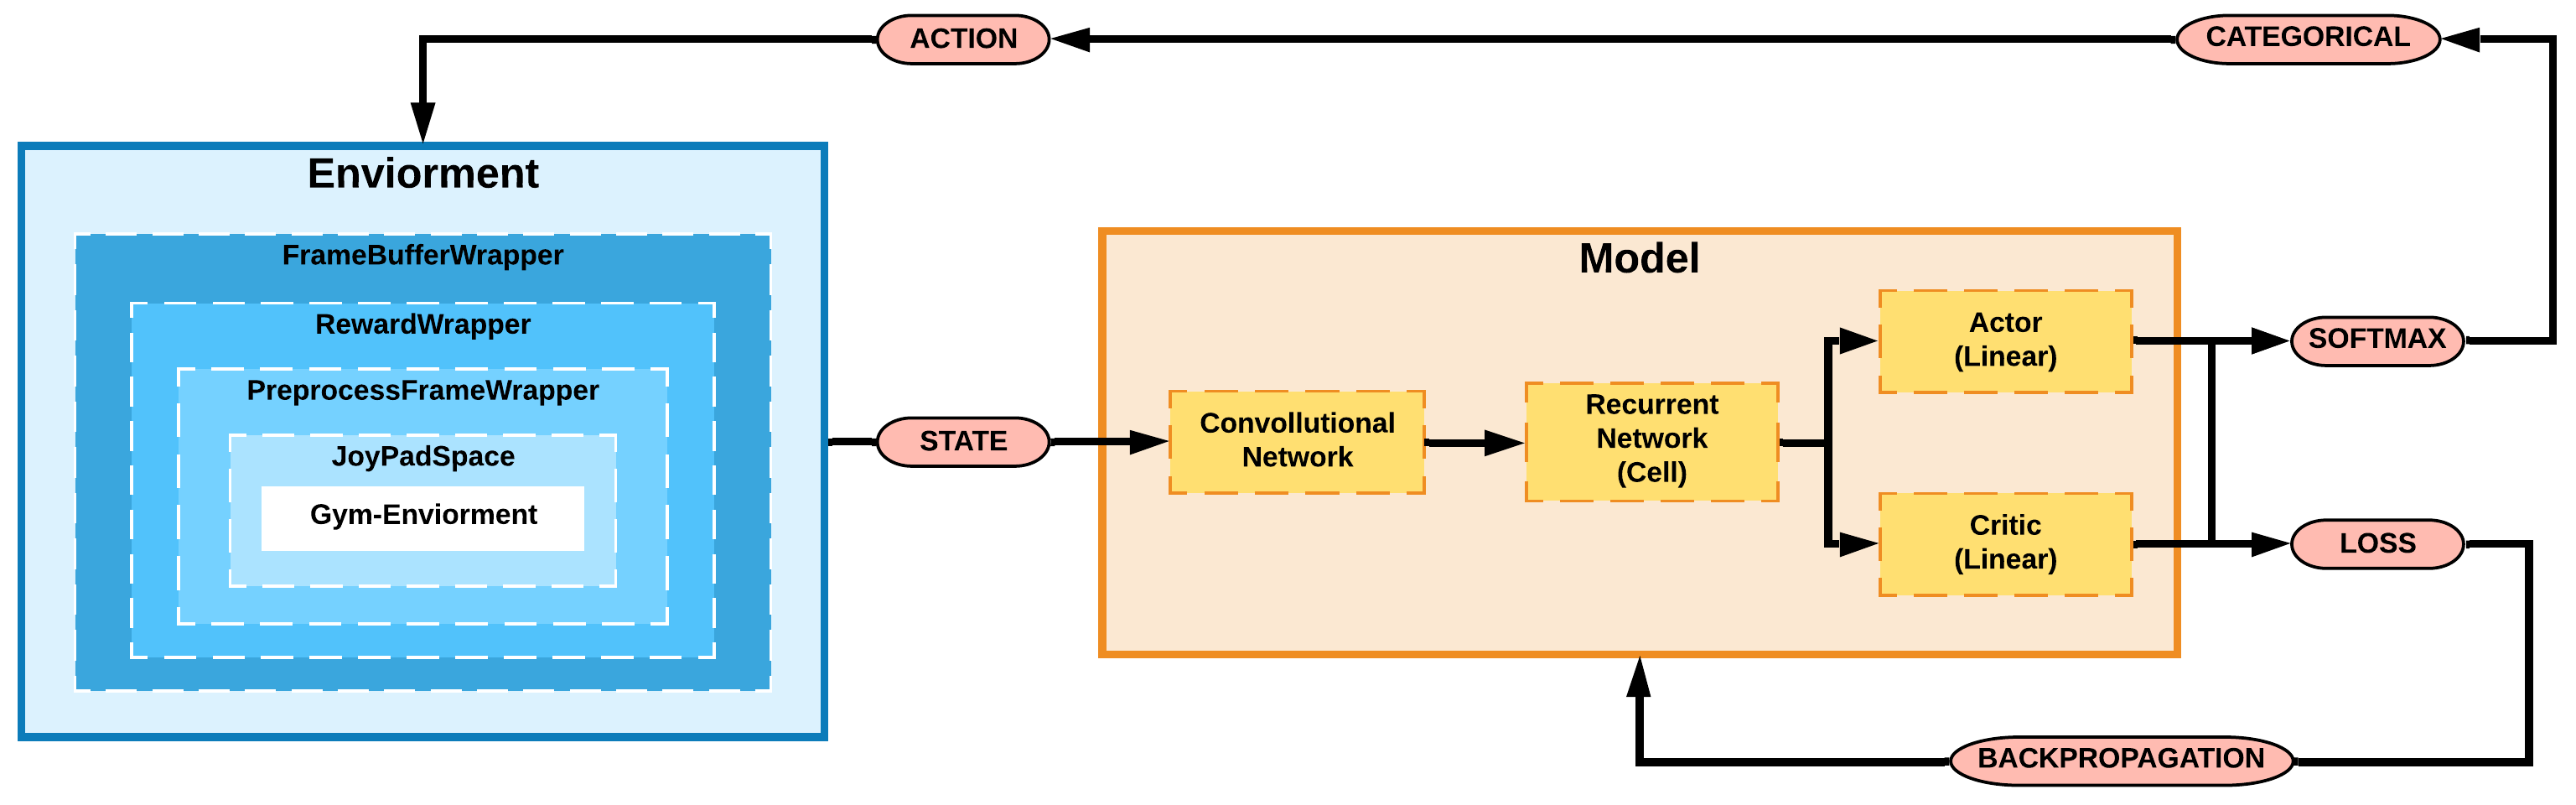
\includegraphics[angle=90,scale=0.11]{images/Basis_Architektur_c.png}
\caption{Vollständiger Kontext des Modells}
\label{fig:KontextModel}
\end{figure}

\subsection{Hyperparameter}
Für das komplette Experiment wurden im üblichen Wertebereich liegende \textit{Hyperparamter} verwendet:
\begin{equation}
lr\ =\ 0.0001
\end{equation}
\begin{equation}
gamma\ =\ 0.9
\end{equation}
\begin{equation}
beta\ =\ 0.01
\end{equation}

\section{Experiment und Ergebnisse}
Für das folgende Experiment wurden auf Basis der Hardware (vgl. \ref{hardware}) fünf parallel Trainings-Threads gestartet. Diese arbeiteten jeweils eine vorgegebene Anzahl von Epochen ab. Zusätzlich zu den Trainings-Thread, wurde ein Thread gestartet, welcher den aktuellen Zustand des globalen Modells wiederspiegelte. Während des Trainings lief zudem zur Live-Ansicht der Lernergbnisse im Hintergrund der \textit{Tensorboard-Service}.

In den nachfolgenden Abbildungen \ref{fig:x}, \ref{fig:flag} und \ref{fig:reward} sind die Farben jeweils nach der Legende (Abb. \ref{fig:legende}) gewählt. Zusehen sind hier die Ergebnisse nach 3500 Trainingsepisoden bei 5 Trainingsthread für das allererste Super Mario Bros. Level. Insgesamt wurden also 17500 Episoden pro Netzwerk trainiert. Auf den X-Achsen ist die verstrichene Zeit aufgeführt, auf der Y-Achse der für das Diagramm spezifisch erreichte Werte. Die Graphen sind zur besseren Verständlichkeit mit einem Smoothingfaktor von 85\% dargestellt.

\subsection{Direkter Vergleich von Netzwerken}
\label{exp1}
Nachfolgend werden die Ergebnisse der jeweiligen Netzwerke kurz aufgeführt.

\subsubsection{DCN + GRU}\hfill \break
Das \textit{Deep(ish)-Convolutional-Netzwerk} in Kombination mit der \textit{GRU-Zelle} erwies sich als am schnellsten lernende Kombination. Bereits nach ca. 27 Minuten wurde das Ziel erstmalig erreicht; das Lernziel war hier anschließend nach ca. 34 Minuten erreicht.

Im weiteren Verlauf verließ dieses Netzwerk allerdings zweimal den zielführenden Weg für ca. 3 Minuten und Aufgrund des Zeitpunkt nicht näher definierbaren Zeitrahmen, innerhalb des ca. einstündigen Trainingszeitraum.

Auffällig für dieses Netzwerk ist die frühe stabile starke Lernperformance mit einem Vorsprung von bis zu ca. 5 Minuten vor den anderen Kombinationen.

\subsubsection{CNN + GRU}\hfill \break
Das einfache \textit{CNN} in Kombination mit der\textit{GRU-Zelle} erwies sich hingegen als langsam lernende Kombination. Auch wenn nach 29 Minuten das Ziel erstmalig erreicht wurde, wurde das Lernziel erst nach ca. 35 Minuten erreicht.

Im weiteren Verlauf verließ dieses Netzwerk allerdings dreimal den zielführenden Weg für insgesamt 7 Minuten.

Auffällig für dieses Netzwerk ist die bereits früh auftauchende Instabilität.

\subsubsection{CNN + LSTM}\hfill \break
Als äußerst langsam lernendes Netzwerk erwies sich die Kombination aus naiven \textit{CNN} mit \textit{LSTM-Zelle}. Auch wenn nach 27 Minuten das Ziel erstmalig erreicht werden konnte, wurde das Lernziel erst nach ca. 36 Minuten erreicht.

Im weiteren Verlauf erwies es sich zudem als tendenziell instabil und wich dreimal von zielführenden Weg ab für insgesamt ca. 5 Minuten.

\subsubsection{DCN + LSTM}\hfill \break
Die Kombination aus Deep(ish)-Convolutional-Netzwerk mit \textit{LSTM-Zelle} erwies sich als langsamstes lernendes Netzwerk. Nach ca. 33 Minuten wurde das Ziel erstmalig erreicht, nach 39 Minuten wurde das Lernziel erreicht.

Im weiteren Verlauf verließ dieses Netzwerk kein einziges Mal den zielführenden Weg.

Auffällig für diese Kombination ist die für den Trainingszeitraum perfekte Stabilität und die ca. 58 Minuten auftrettende wachsende Führung des insgesamt erreichten Rewardes.

\begin{figure}[hbt!]
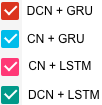
\includegraphics[scale=0.5]{images/legende.png}
\caption{Legende für die Ergebnisse}
\label{fig:legende}
\end{figure}

\begin{figure}[hbt!]
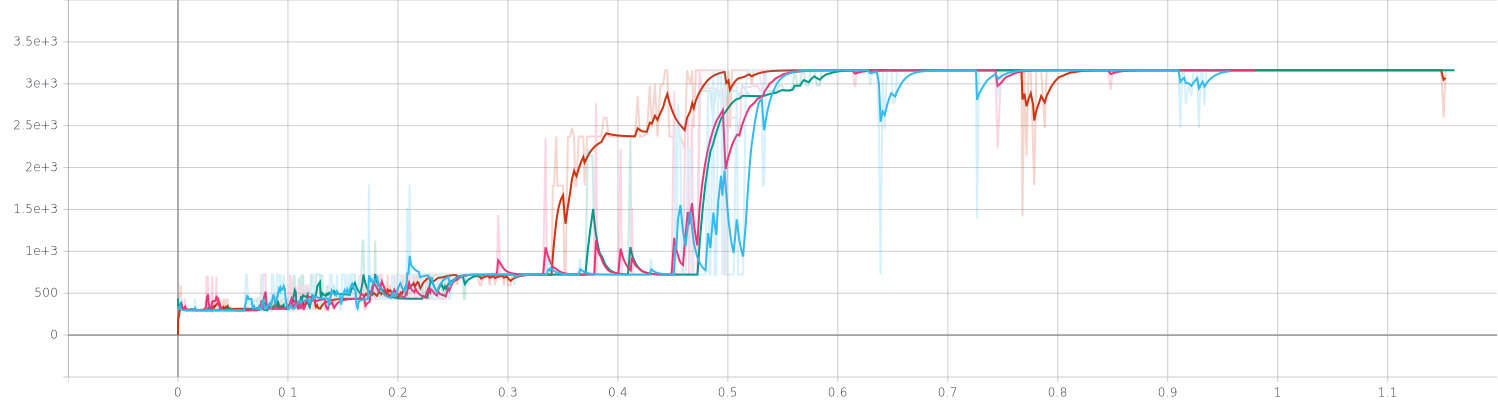
\includegraphics[angle=90,scale=0.385]{images/x_position.png}
\caption{Ergebnis: Erreichte X-Position}
\label{fig:x}
\end{figure}

\begin{figure}[hbt!]
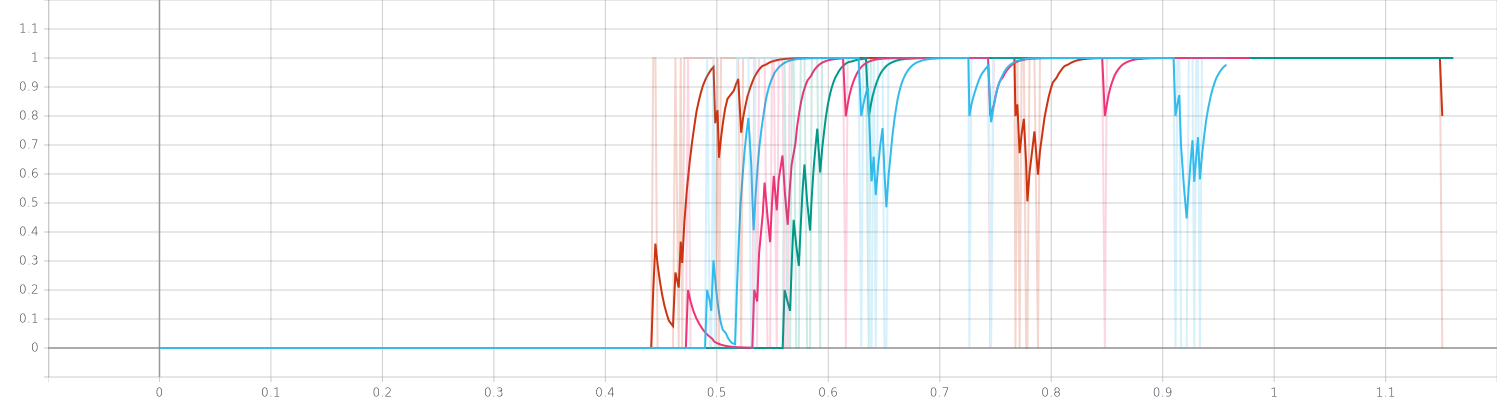
\includegraphics[angle=90,scale=0.385]{images/flag.png}
\caption{Ergebnis: Erreichte Flagge}
\label{fig:flag}
\end{figure}

\begin{figure}[hbt!]
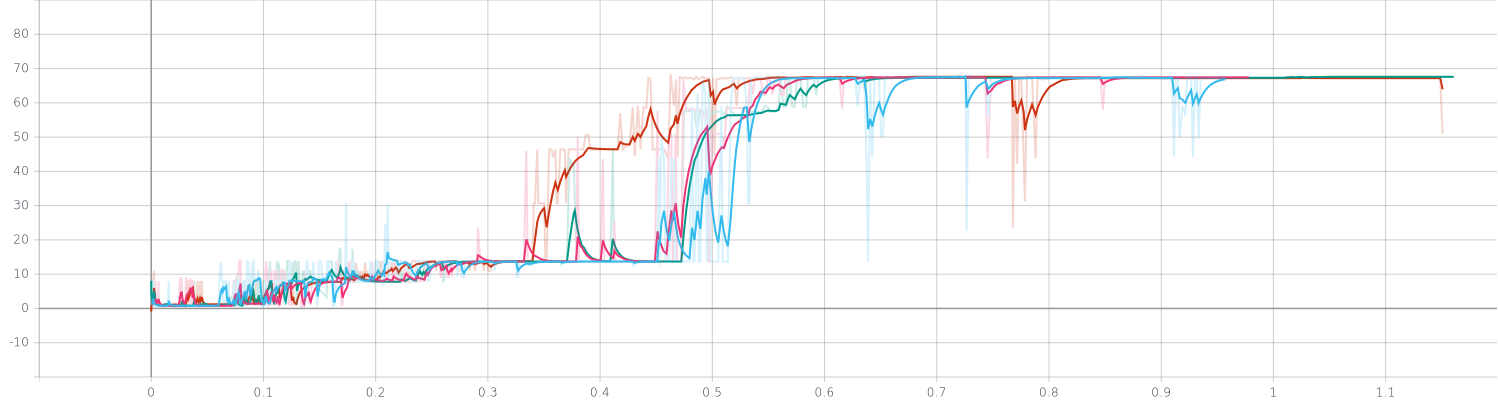
\includegraphics[angle=90,scale=0.385]{images/sum_reward.png}
\caption{Ergebnis: Insgesamt erreichter Reward}
\label{fig:reward}
\end{figure}

\subsection{Zwischenfazit}

Ausgehend von vorherigen Test in Kombinationen mit weiteren kleineren Experimenten lässt sich feststellen, dass die Lernstabiltät eine übergeordnete Rolle zum lösen des SMB-Problemes aufweist. Denn testet man schnelle Netzwerke wie die Kombination von \textit{DCN} und \textit{GRU-Zelle} so lässt sich feststellen, dass nicht immer das Ziel erreicht werden kann, ähnlich gut bzw. schlecht verhalten sich die anderen beiden Netzwerkarchitekturen. Hierfür ist u.a. die Struktur der Level, bestehend aus Sackgassen, Engstellen, Fallen, Sprungpassagen oder ähnliche in Kombination mit dem Rewardshaping verantwortlich.

Vergleicht man die Aufnahmen der Trainingsdurchgänge (zu finden im Projektrepository \cite{selfgit}) so fällt auf, dass es auch nach dem Training für alle Netzwerkkombination noch Verbesserungspotential innerhalb von wenigen Millisekunden besteht, geschuldet dadurch das Mario an einzelnen Hindernissen kurz zum stoppen kommt.

Abschließend wurden weitere Test mit dem erfolgversprechendem Netzwerk, bestehend aus \textit{Deep(ish)-Convolutional-Netzwerk} und \textit{LSTM-Zelle}, durchgeführt um weitere Aussagen hinsichtlich der Lernperformance zu treffen bzw. zu bestätigen.

\subsection{Weiterführende Beobachtungen}

Nachfolgend werden die restlichen drei Level der ersten SMB-Welt mit \textit{DCN} und \textit{LSTM-Zellen} aufgeführt.

\subsubsection{Level 2}\hfill \break

Beim zweiten SMB-Leve erreichte keines der Netzwerkkombinationen aus dem ersten Experiment (vgl. \ref{exp1}) das Ziel. Alle blieben an der selben Stelle hängen: Einer Sackgasse, wo der eigentliche Lösungsweg durch mehrere Gegner für eine geringe Zeit blockiert wird.

Ursächlich hierfür ist das \textit{Rewardshaping}, welches den Lösungsweg nicht mit längeren Wartezeiten definiert. Es zeigte sich, dass mit einem weitestgehend randomisierten Reward diese Stelle über einen entsprechend längeren Zeitraum von den meisten Kandidaten lösbar war.

\subsubsection{Level 3}\hfill \break

Nachfolgend werden die Ergebnisse aus Abbildung \ref{fig:w1s3} kurz analysiert. Es wurden 5 Threads mit jeweils 2500 Episoden trainiert.

Level 3 besteht hierbei im wesentlich aus Sprungpassagen unterschiedlicher Schwierigkeitsgrade, welche dem ersten Level tendenziell ähnelt, wodurch sich die Ähnlichkeit der Lernperformance erklären lässt.

Nach ca. 31 Minuten wurde erstmalig das Ziel erreicht, nach weiteren 3 Minuten war das Lernziel erreicht. Ähnlich wie in dem vorherigen Experiment fällt die Lernstabilität auf. Es ist auch anzumerken, dass hier ebenfalls nach Erreichen des Lernzieles ein weiterer Lernerfolg messbar ist in Form des insgesamt verdienten Rewardes.

\begin{figure}[hbt!]
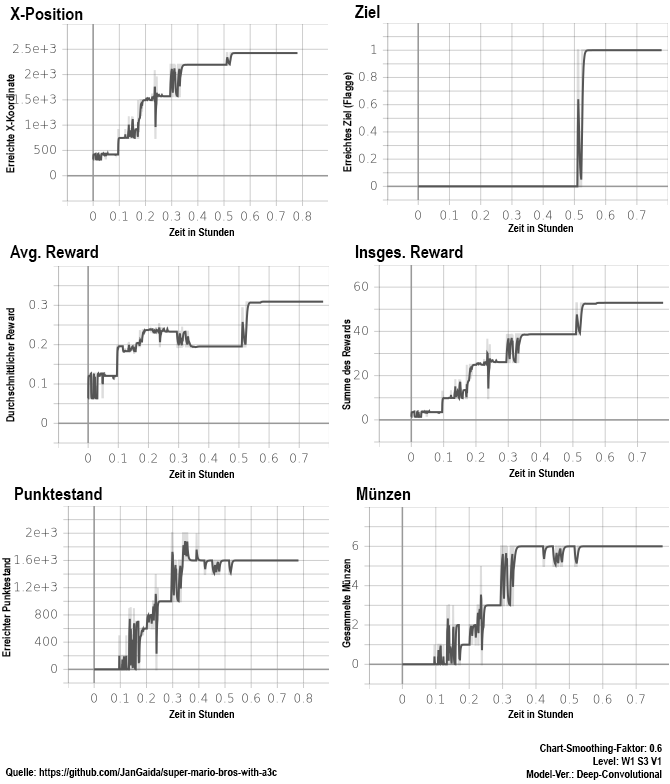
\includegraphics[width=\columnwidth]{images/stats_w1s3v0_dcn.png}
\caption{Ergebnis: Welt 1 Level 3}
\label{fig:w1s3}
\end{figure}

\subsubsection{Level 4}\hfill \break

Nachfolgend werden die Ergebnisse aus Abbildung \ref{fig:w1s4} kurz analysiert. Es wurden 5 Threads mit jeweils 7500 Episoden trainiert.

Das Level 4 beinhaltet das erste Auftreten des \textit{Bowser} Gegners und besteht aus einigen sehr schwierigen Passagen wie bspw. schwierigen Sprungpassagen, tödlichen Sackgassen, feindliche Projektile und sich bewegende Hindernisse.

Nach ca. 54 Minuten wurde das Ziel erstmalige erreicht, nach ca. 72 Minuten stellte sich das Lernziel ein, unterbrochen durch einen ca. 5 Minütigen Misserfolg.

Auffällig ist hierbei die relativ instabile Lernrate zu Beginn des Trainings, welche auf die Schwierigkeit des Levels zurückzuführen ist. Auffällig ist auch die minimal instabile Rewardrate nach dem Erreichen des Lernzieles.

\begin{figure}[hbt!]
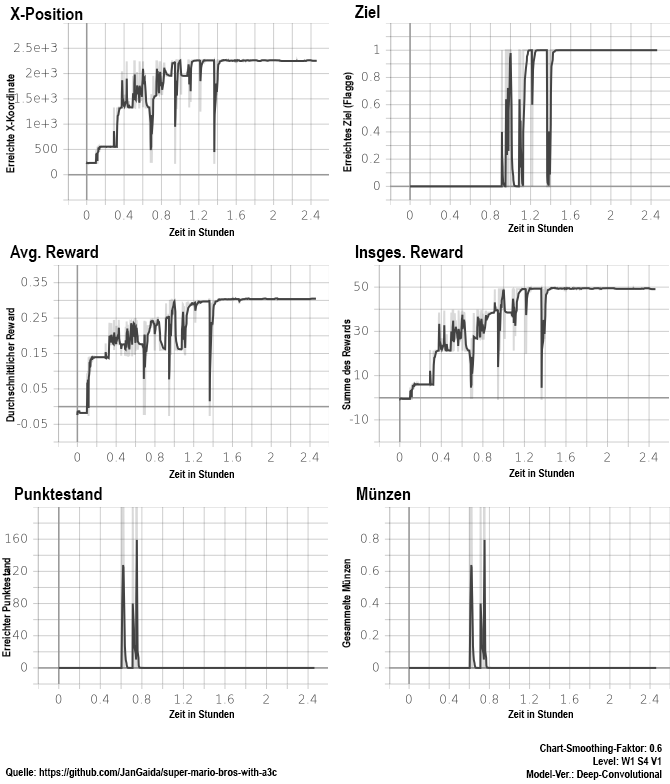
\includegraphics[width=\columnwidth]{images/stats_w1s4v0_dcn.png}
\caption{Ergebnis: Welt 1 Level 4}
\label{fig:w1s4}
\end{figure}

\section{Resümee}
Fasst man die Ergebnisse dieser Studienarbeit also zusammen, lässt sich zunächst erst einmal feststellen, dass SMB für viele RL-Algorithmen eine Herausforderung darstellt. Es lässt sich zwar vermuten, dass mit leistungsstärkerer Hardware noch schneller das Lernziel erreicht werden kann, dennoch wird aufgrund der tendenziell geringen Explorationsrate bei den getesteten RL-Algorithmen nicht der bestmöglichste Lösungwegs zeitnah gefunden.

Für die Suche nach diesen bestmöglichen Lösungweg erwies sich die Stabilität des Lernerfolgs als äußerst wichtig, auch wenn diese dazu führt, dass das eigentliche Lernziel später erreicht wird. Desweiteren lässt sich feststellen, dass diese Stabilität des Lernerfolgs auch dazuführen kann, dass vorallem schwierige Passagen schneller gelöst werden kann.

Hinsichtlich der verwendeten neuronalen Schichten erwies sich die GRU-Zelle als schnell lernfähig, wohingegen die LSTM-Zelle sich als stabil erwies. Hinsichtlich des CNN erwies sich eine in Branchen unterteilte Variante performanter als eine Serielle Variante.

Auch wenn für ein aussagekräftiges Studienergebnis weitere Tests notwendig sind, lassen doch wichtige Charakteristika der verwendetet neuronalen Netzwerkarchitekturen feststellen, welche wiederum aktuelle Forschungsgebiete streifen.

\bibliography{citations}

\listoffigures

\end{document}

\endinput
